
\begin{itemize}
    \iitem{state as vector of numbers $(0, 0, 0, 0, 1, 1, 1, 1, \ldots)$}
    \iitem{permutations behave as}
    \begin{equation*}
        f_0 = \begin{pmatrix}
            0 & 1 & 2 & 3 & \ldots\\
            0 & 1 & 19 & 17 & \ldots\\
        \end{pmatrix}
    \end{equation*}
\end{itemize}

\begin{figure}[h]
    \centering
    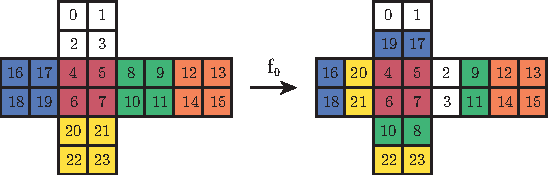
\includegraphics{imgs/pAsset 1.pdf} \vspace{5mm}
    \caption{Example of permutation, code \href{https://www.kaggle.com/code/marksix/visualize-allowed-moves}{here}}
    %\label{fig:}
\end{figure}
